\chapter{Specyfikacja}

\section{Architektura systemu}
\begin{figure}[h!]
	\centering
	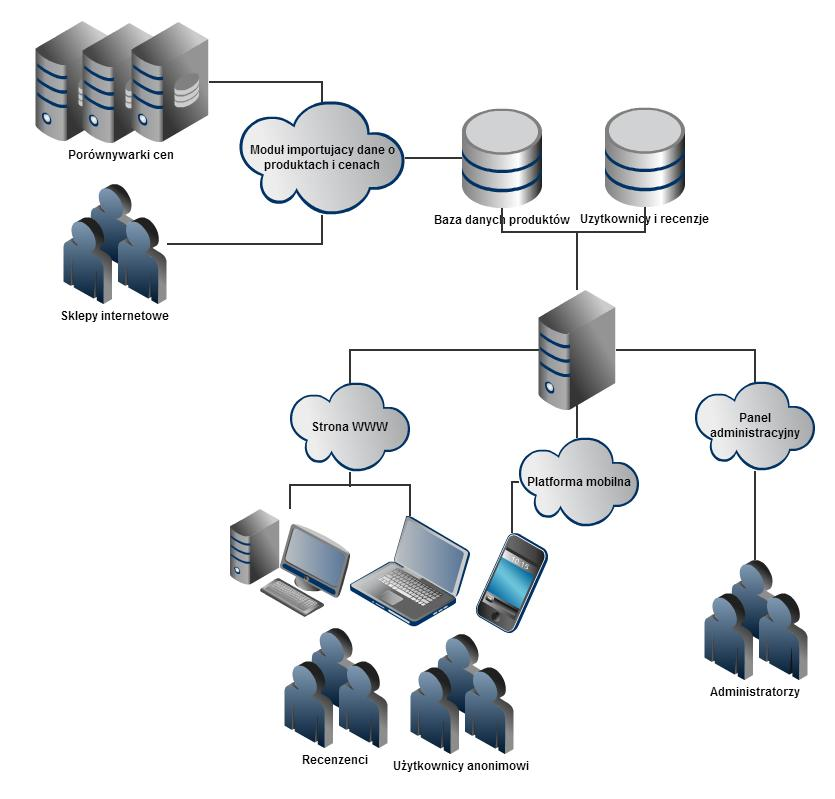
\includegraphics[scale=0.5]{images/architektura.jpg}
	\caption{Architektura systemu}
\end{figure}

\section{Warstwy implementacyjne}
\begin{figure}[h!]
	\centering
	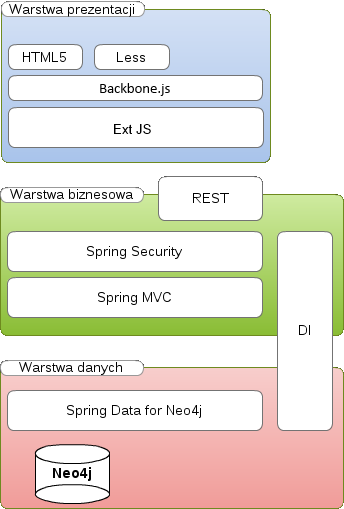
\includegraphics[scale=0.9]{images/warstwy.png}
	\caption{Warstwy implementacyjne}
\end{figure}

\section{Struktura programowa}
\begin{figure}[h!]
	\centering
	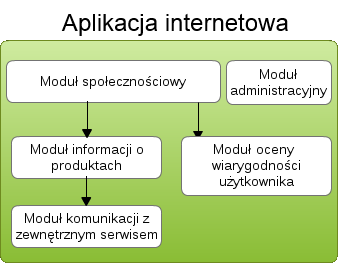
\includegraphics[scale=0.9]{images/modules.png}
	\caption{Struktura programowa}
\end{figure}

\section{Wymagania funkcjonalne}
\begin{figure}[h!]
	\centering
	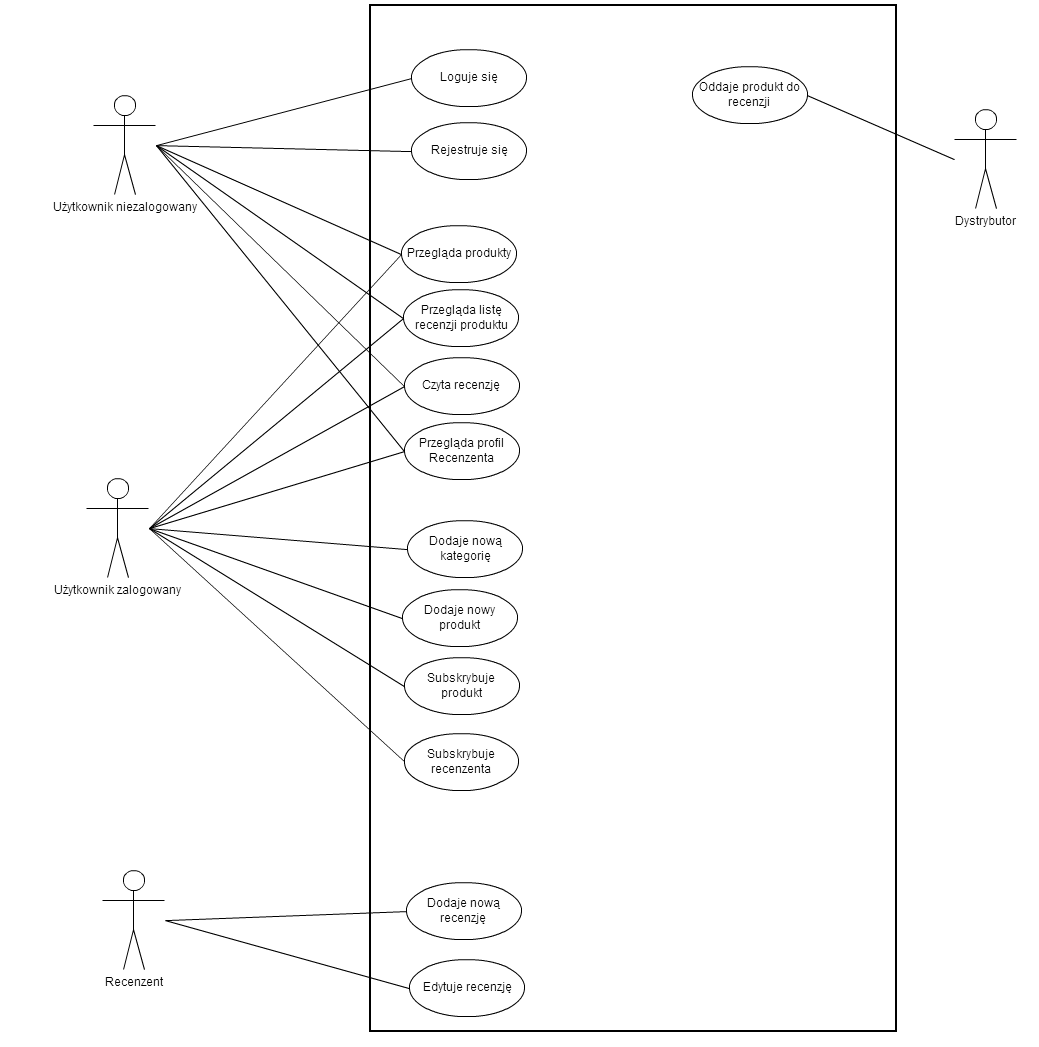
\includegraphics[scale=0.4]{images/funkcjonalne.png}
	\caption{Wymagania funkcjonalne}
\end{figure}

\section{Wymagania pozafunkcjonalne}
\begin{itemize}
\item System powinien działać prawidłowo na przeglądarkach Chrome, Opera, Safari, Firefox oraz Internet Explorer
\item Dane w systemie powinny być przechowywane w grafowej bazie danych
\item Kod źródlowy powinien być stworzony zgodnie ze standardami wybranego języka
\item Maksymalny czas odpowiedzi systemu powinien być mniejszy niż 3 sek.
\item Hasła użytkowników powinny być przechowywane w postaci zaszyfrowanej
\item System powinien uniemożliwiać łatwe podszycie się pod innego użytkownika 
\item Dane powinny być pobierane do systemu za pośrednictwem zewnętrznego API
\item Źródło danych powinno być w łatwy sposób podmienialne
\item System powinien posiadać modularną strukturę, pozwalającą na łatwą podmianę np. frontendu
\end{itemize}

\section{Aktorzy i charakterystyka użytkowników}
\begin{figure}[h!]
	\centering
	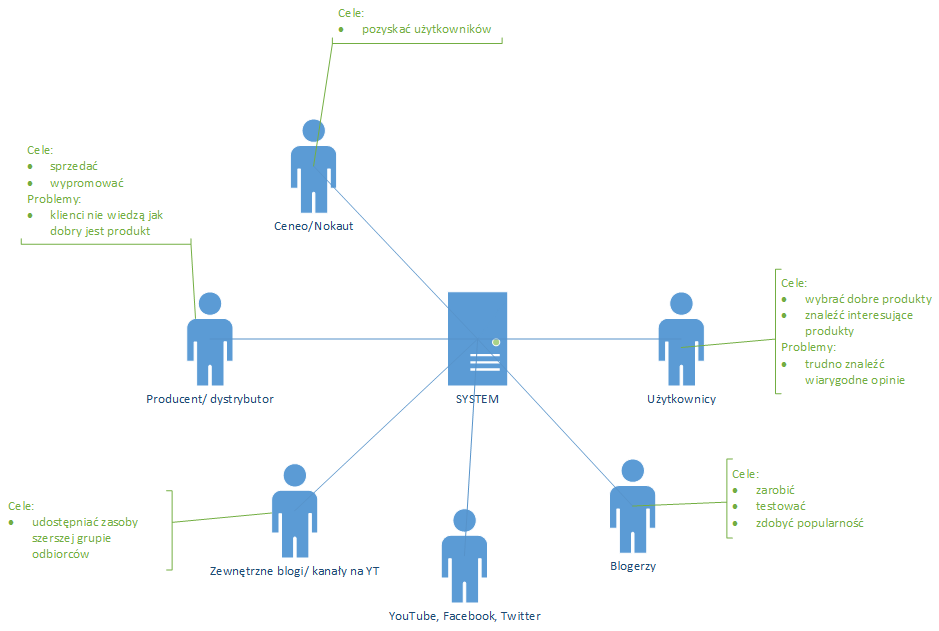
\includegraphics[scale=0.65]{images/Strony_cele.png}
	\caption{Aktorzy i charakterystyka użytkowników}
\end{figure}